\section{Recursos principals del bloc Fonts de Dades}

    \paragraph{}
    Aquest bloc de l'arbre familiar destaca pels recursos Col·lecció i Font de Dades, que s'utilitzen per certificar la veracitat de les dades referents a les persones que es poden trobar a l'arbre familiar o les relacions que les uneixen.

    Aquest bloc és realment important, ja que és l'encarregat de garantir la integritat de les dades i per tant, d'assegurar que la informació continguda a l'arbre familiar de FamilySearch sigui usable i interessant pels usuaris de l'aplicació.

    Així doncs, les fonts de dades són utilitzades per demostrar que un esdeveniment en concret va succeir o que les dades de la persona citada són les mateixes que aquelles redactades en els documents oficials.

    Les fonts de dades s'agrupen i emmagatzemen en col·leccions i cada persona o relació, disposa d'un recurs que actua com intermediari per relacionar-los amb les fonts de dades. Com sempre, els enllaços explícits entre els diferents recursos es realitzen mitjançant els enllaços hypermedia. La imatge~\ref{img:sourcesBloc} ofereix una vista de com s'estructuren i relacionen els diferents recursos del bloc Font de Dades.

    \begin{figure}[h]
        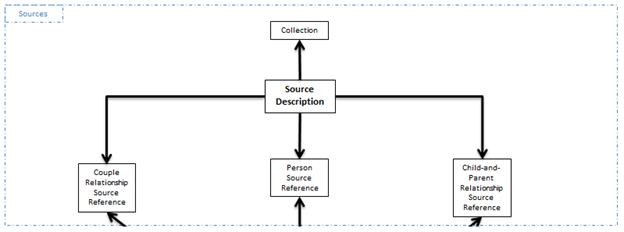
\includegraphics{05/07_sourcesCore}
        \centering
        \caption{El bloc de l'arbre familiar relatiu a les fonts de dades}\label{img:sourcesBloc}
    \end{figure}

    Podreu observar també, a les taules que representen l'estructura dels recursos, que a vegades, per la columna que marca el format de dades d'un paràmetre, aquest es troba especificat entre els caràcters `[' i `]'. Aquesta terminologia s'utilitza per indicar que aquest paràmetre és en realitat un recurs o objecte de dades diferent inclòs dins del recurs estudiat.

    També s'observarà que sovint, els recursos exposats, hereten dades d'altres recursos i en els casos que aquests siguin rellevants, se n'exposarà l'estructura a l'apartat `Altres recursos interessants', més endavant en la memòria.

    \subsection{El recurs Col·lecció (Collection)}

    \paragraph{}
    Aquest recurs representa una col·lecció o agregació, de fonts de dades de caràcter genealògic.

    Aquestes dades poden fer referència tant a les dades internes de FamilySearch, com als registres bolcats per tercers a les bases de dades. Per tal d'ajudar al lector a fer-se una idea, una col·lecció podria ser per exemple el conjunt de fonts de dades que conformen l'arbre familiar.

    La taula~\ref{res:collection} mostra els paràmetres que aquest recurs incorpora i també hereta els paràmetres dels recursos Enllaços Hypermedia i Dades Extensibles que poden ser trobats a l'apartat `Altres recursos interessants'.

    \begin{center}
             \csvreader[
                separator=comma,
                before table=\sffamily\small,
                longtable={p{2cm-2\tabcolsep}p{3.5cm-2\tabcolsep}p{8.5cm-2\tabcolsep}},
                table head={\caption{Paràmetres del recurs Col·lecció}\label{res:collection}\\\toprule%
                    \headentry{m{2cm-2\tabcolsep}}{Paràmetre}
                    & \headentry{m{3.4cm-2\tabcolsep}}{Format de Dades}
                    & \headentry{m{8.5cm-2\tabcolsep}}{Descripció}\\\midrule},
                late after line=\\\midrule,
                late after last line=\\\bottomrule,
             ]
             {./tables/05/05_sources/collection.csv}
             {param=\param,format=\format,desc=\desc}
             {\param&\format&\desc}
     \end{center}

    \subsection{El recurs Contingut de la Col·lecció (CollectionContent)}

    \paragraph{}
    Aquest recurs conté informació específica sobre la col·lecció a la que fa referència. Serveix per  comprendre millor l'estat actual de migració de la col·lecció a les bases de dades de FamilySearch, així com informació sobre el contingut que aquesta aporta.

    La taula~\ref{res:collectionContent} mostra els paràmetres inclosos en el recurs, que a la vegada hereta els paràmetres dels recursos Enllaços Hypermedia i Dades Extensibles que poden ser trobats a l'apartat `Altres recursos interessants'.

    \begin{center}
             \csvreader[
                separator=comma,
                before table=\sffamily\small,
                longtable={p{2cm-2\tabcolsep}p{3.5cm-2\tabcolsep}p{8.5cm-2\tabcolsep}},
                table head={\caption{Paràmetres del recurs Contingut de la Col·lecció}\label{res:collectionContent}\\\toprule%
                    \headentry{m{2cm-2\tabcolsep}}{Paràmetre}
                    & \headentry{m{3.4cm-2\tabcolsep}}{Format de Dades}
                    & \headentry{m{8.5cm-2\tabcolsep}}{Descripció}\\\midrule},
                late after line=\\\midrule,
                late after last line=\\\bottomrule,
             ]
             {./tables/05/05_sources/collectionContent.csv}
             {param=\param,format=\format,desc=\desc}
             {\param&\format&\desc}
     \end{center}

    \subsection{El recurs Atribució (Attribution)}

    \paragraph{}
    El recurs Atribució s'utilitza en més llocs que les fonts de dades, però com que juga un paper especialment important en aquest, hem decidit incloure'l dins d'aquesta secció.

    Aquest recurs conté principalment paràmetres que permeten descriure qui, quan i perquè, va ser realitzada una contribució o modificació sobre les dades.

    Els paràmetres d'aquest recurs són descrits a la taula~\ref{res:attribution}, que també hereta els paràmetres del recurs Dades Extensibles, que pot ser trobat a l'apartat `Altres recursos interessants'.

    \begin{center}
             \csvreader[
                separator=comma,
                before table=\sffamily\small,
                longtable={p{2cm-2\tabcolsep}p{3.5cm-2\tabcolsep}p{8.5cm-2\tabcolsep}},
                table head={\caption{Paràmetres del recurs Atribució}\label{res:attribution}\\\toprule%
                    \headentry{m{2cm-2\tabcolsep}}{Paràmetre}
                    & \headentry{m{3.4cm-2\tabcolsep}}{Format de Dades}
                    & \headentry{m{8.5cm-2\tabcolsep}}{Descripció}\\\midrule},
                late after line=\\\midrule,
                late after last line=\\\bottomrule,
             ]
             {./tables/05/05_sources/attribution.csv}
             {param=\param,format=\format,desc=\desc}
             {\param&\format&\desc}
     \end{center}

    \subsection{El recurs Font de Dades (SourceDescription)}

    \paragraph{}
    Aquest recurs defineix una font de dades i n'emmagatzema tota la informació que la caracteritza. Les fonts de dades formen part d'una col·lecció i es troben relacionades a ella mitjançant enllaços hypermedia.

    La millor forma d'explicar aquest recurs és comprendre'n els paràmetres i aquests s'exposen a la taula~\ref{res:sourceDescription}. El recurs Font de Dades també hereta els paràmetres dels recursos Enllaços Hypermedia i Dades Extensibles, que poden ser trobats a l'apartat `Altres recursos interessants'.

    \begin{center}
             \csvreader[
                separator=semicolon,
                before table=\sffamily\small,
                longtable={p{2cm-2\tabcolsep}p{3.5cm-2\tabcolsep}p{8.5cm-2\tabcolsep}},
                table head={\caption{Paràmetres del recurs Font de Dades}\label{res:sourceDescription}\\\toprule%
                    \headentry{m{2cm-2\tabcolsep}}{Paràmetre}
                    & \headentry{m{3.4cm-2\tabcolsep}}{Format de Dades}
                    & \headentry{m{8.5cm-2\tabcolsep}}{Descripció}\\\midrule},
                late after line=\\\midrule,
                late after last line=\\\bottomrule,
             ]
             {./tables/05/05_sources/sourceDescription.csv}
             {param=\param,format=\format,desc=\desc}
             {\param&\format&\desc}
     \end{center}


    \subsubsection{L'enumeració resourceType}

    L'enumeració resourceType segueix l'estructura de definició GEDCOMX. Com a tal, els valors possibles per l'enumeració segueixen la pauta:

    http://gedcomx.org/ + `resourceType'

    La següent taula mostra els possibles valors per l'enumeració resourceType.

    \begin{center}
        \csvreader[
           no head,
           separator=comma,
           table head={\caption{Valors possibles per l'enumeració resourceType}\label{enum:resourceType}},
           before table=\sffamily\small,
           longtable={|p{3cm}|p{3cm}|p{3cm}|},
           column count=3,
           late after head=\\\hline,
           late after line=\\\hline,
           late after last line=\\\hline,
        ]
        {./tables/05/05_sources/resourceType.csv}
        {1=\one,2=\two,3=\three}
        {\one&\two&\three}
    \end{center}

    \subsection{El recurs Referència a la Font de Dades (SourceReference)}

    \paragraph{}
    Aquest recurs s'utilitza per fer de pont entre els diferents recursos de l'arbre fa\-mi\-liar, que contenen informació genealògica i les fonts de dades que l'han proporcionat.

    Com s'ha pogut veure en la imatge~\ref{img:sourcesBloc}, que obria el bloc de Fonts de Dades, el recurs Referència a la Font de Dades aplica tant a les relacions familiars, com a les persones. De la mateixa forma, aquest recurs també es veu utilitzat per relacionar diferents Fonts de Dades entre elles.

    A part dels paràmetres que conformen aquest recurs i que es mostren a la taula~\ref{res:sourceReference}, també hereta els paràmetres dels recursos Enllaços Hypermedia i Dades Extensibles, que poden ser trobats a l'apartat `Altres recursos interessants'.

    \begin{center}
             \csvreader[
                separator=semicolon,
                before table=\sffamily\small,
                longtable={p{2cm-2\tabcolsep}p{3.5cm-2\tabcolsep}p{8.5cm-2\tabcolsep}},
                table head={\caption{Recurs Referència a la Font de Dades}\label{res:sourceReference}\\\toprule%
                    \headentry{m{2cm-2\tabcolsep}}{Paràmetre}
                    & \headentry{m{3.4cm-2\tabcolsep}}{Format de Dades}
                    & \headentry{m{8.5cm-2\tabcolsep}}{Descripció}\\\midrule},
                late after line=\\\midrule,
                late after last line=\\\bottomrule,
             ]
             {./tables/05/05_sources/sourceReference.csv}
             {param=\param,format=\format,desc=\desc}
             {\param&\format&\desc}
     \end{center}

